\part{Refactor (To be deleted)}
\section{Risikoanalys}

Entscheidungen für \gls{p_NFM} müssen zum einen direkt oder indirekt getroffen werden.
Direkt, wenn sich z.B. für Kindergarten, Schule, Kleidung entschieden wird. Indirekt, wo wir als Familie leben.\\

Hier wird primär von Geld Ressourcen gesprochen. Ressourcen vor allem in den ersten Jahren werden mehr benötigt. Im direkten Fall, wenn z.B. Kleidung, Schulsachen, Spielsachen für \gls{p_NFM} benötigt werden. Im indirekten Fall, wenn z.B. die Miete, Essen, Aktivitäten mit für \gls{p_NFM} bezahlt werden.

Beim Thema Betreuung ist damit gemeint, dass hier Zeit und Aufmerksamkeit benötigt wird, für Themen welche für \gls{p_NFM} wichtig sind, welche aber sie nicht aus alleiniger Kraft umgesetzt bekommt oder wir in der \gls{p_ER} ein hohes Risiko sehen, dass \gls{p_NFM} Schaden nimmt.\\

Bei diesen drei Bereichen ist \gls{p_NFM} entweder auf die \gls{p_E}, die Familie angewiesen oder diese leitete oder schränkt Bereiche im Leben von \gls{p_NFM} ein. Hier wird angenommen, um \nameref{NFM_O_1} langfristig zu erreichen, muss die \gls{p_ER} in der \gls{p_EKB} an Relevanz verlieren, welche das Ungleichgewicht absenkt, und mehr Raum für \nameref{NFM_O_3} ergibt.\\

%TODO: Wie: Spektrum der Rolle

Was es bedeutet, Dein eigenes Leben zu leben, steht immer zu debatte. Wir geben uns aber Mühe, so transparenz wie möglich, es aufzuzeigen, welche Eckpfeiler wir als wichtig erachten, dass Du Dein eigenes Leben für Dich, in unsere Familie und der Gesellschaft leben kannst.

\subsection{Kontext: Eigenen Zielsetzunng}

Mein Ziel ist, dass ich eine tolle Familie und super Freude habe.\\

Eine \textit{tolle Familie} für jedes Familienmitglied zu schaffen.\\

\subsection{Eigener Bedarf}

% Teilziel
%% Frau ist glücklich, ohne Restriktion
%% Erkennung der eigenen Einschränkungen

Was im Prozess der Niederschrift dieser Strategie sich offenbart hat, ist, dass mit diesem Formulierung, keine passende externe Metrik gemeint ist, sondern ein interner, persönlicher Gefühlszustand angestrebt ist: Das Gefühl von 
\textit{sozialem Vertrauen},
 \textit{Aufgehobenheit}
  und \textit{gemeinsamen Genuss des $"$Lebens$"$}. 
Besonders im Bezug zu meiner Frau benötige ich das Gefühl von Vertrauen. Das Vertrauen, sich nicht Gedanken machen zu müssen, ob die Person ihr Leben im Griff hat und ob sie sich das von einem einfordert, was sie benötigt, um selbst glücklich zu sein. Das Gefühl aufgehoben zu sein, erfordert vermutlich ein sehr persönlichen Zustand um einen herum. Mein Ziel damit ist, dass man seine Vasseten der Persönlichkeit ausleben kann und soll. Einige Vassetten sind vermutlich von direkte positiver Bedeutung für die anderen Familienmitglieder, andere weniger. Für unser Familienzusammenleben ist es unabdingbar, dass über die eignen Ausprägungen nachgedacht werden, welche einem selbst und andere keinen Mehrwert bringen.\footnote{
	Theoretischer Vermerk: Über Ausprägungen der Persönlichkeit, welche einem selbst ein gutes Gefühl geben, aber die sozialen Kosten so hoch sind, dass sie in anderen Bereichen des eigenen Lebens zu viel Einschränkungen bringen, muss ebenso abgewägt werden.
} Das Gefühl, dass die positiven, wie die nervigen Ausprägungen seiner Persönlichkeit nicht eingestellt werden müssen, ist mit Aufgehobenheit gemeint. Ist diese emotionale Basis gegeben, ist die Annahme, dass die bestmöglichste Chance gemeinsam so viel wie möglich im Leben zu erleben und genießen.

\section{Spielfeld Familie *}
% Chapter zum Ausprobieren
Um die Zielsetzung zu erreichen, wird sich dem Werkzeug einer \textit{Strategie} bedient, siehe \nameref{Appendix_Erlaeuterung_Strategie}.

\subsection{Emotionale Lage der Familie}

Eine der treibenden Einflussfaktoren auf die eigene Zufriedenheit ist die emotionale Lage der eigenen Familienmitglieder. Diese kann zum einen durch einen selbst gestört werden, welche sich dann wieder auf einen selbst auswirkt, zum anderen durch externe Faktoren beeinflusst werden, welche dann sich auf eine selbst wieder auswirken.


% Identifizierung der Akteure
In der Dynamik im Umgang mit ihnen lassen sich zwei Mechanismen identifizieren, welche relevant in der Kommunikation und Zielausrichtung:
\begin{itemize}
	\item Die Einschätzung des aktuellen Gefühlszustandes des jeweiligen Familienmitgliedes.
	\item und die Antizipierung, wie dieses sich ändert, durch den Einfluss des eigenen Verhaltens.
\end{itemize}
Diese Mechanismen haben jedoch Restritkionen: Es ist nicht immer ersichtlich, ob die erste Einschätzung die richtige war oder nur die Einwirkung durch das eigenen Verhalten nicht den antizipierten Änderungen hervorgerufen hat. Ebenso besteht die Annahme, das basierend an den Randbedingungen es nicht immer möglich ist, einen Einfluss auf den Gefühlszustand zu haben, welchen man selbst sich für die andere Person wünscht.\footnote{
	Loser Gedanke: Dieser rührt daher, dass die andere Person ein externer Faktor für einen darstellt, und diese einen selbst beeinflussen. Ändert sich der externe Faktor, ändert sich das eigenen Gefühl.
}
% Besondere Einwirkung auf NFM
Bei \gls{p_NFM} besteht die Schwierigkeit, dass wir, als Eltern, direkten Einfluss auf die Gefühls und emotionalen Entwicklung von \gls{p_NFM} haben:
\begin{itemize}
 	\item Umgang und Erkennung des persönlichen Affekt Zustandes \footnote{
 		Affect is a combination of two feelings: valence and arousal, see \cite{Feldman-Barrett.Lisa}
 		}
 	\item Beeinfluss direkt und indirekt des Emotionales Lernprozesses
\end{itemize}
Ebenso geben wir vor, was akzeptiertes und nicht akzeptiertes Verhalte vor, besonders in den ersten Jahres.

\subsection{Eigenen Präferenzen}
\subsection{Zielsetzung mit Familie und Freunden}

% Balance finden, zwischen der Formung der emotionalen und Gefühlsentwicklung und der Erkennung, der eigenen Gefühlswelt, welche nicht geändert wird (was wiederum, eine Präferenz von mir ist.)


\section{Zeitstrahl}   

Das Kapitel beschäftigt sich mit dem Thema der Integration eines neuen Familienmitglied in eine bestehende zweier-Familien Struktur. Dabei werden die einzelnen Komponenten unter der Überschrift \gls{p_NFMZ} zusammengefasst.\\

Im folgenden werden drei Schwerpunkte behandelt: 
\begin{itemize}
	\item \gls{p_PEL},
	\item \gls{p_DBS} und
	\item \gls{p_ZK}.

Im ersten Abschnitt, \gls{p_PEL} werden die \gls{p_mpB}\footnote{Beide Eigenschaften werden ebenfalls auf physische Merkmalsausprägen zurückgeführt. In diesem Kontext werden mentale und physische Besonderheiten als Emergenz einer bio-chemischen Merkmalsausprägung bezeichnet.} von Menschen in der Entwicklung eines Neugeborenen bis hin zur einem erwachsenen Menschen \footnote{Der relevante Zeitraum für erwachsene Menschen beträgt hier 18. bis 20. Jahren} aufgedeckt. Es wird dabei nicht auf Vollständigkeit abgezielt, sondern das Ziel verfolgt, gewonnene Informationen über diese Entwicklung unter der Zielsetzung des \gls{p_NFMZ} integrieren zu können.\\

Der Abschnitt \gls{p_DBS} beschäftigt sich mit der Fragestellung, wie die \gls{p_PEL} sich auf die Beziehungen zwischen den bestehenden \gls{p_FM} und dem \gls{p_NFM} auswirken. Der Schwerpunkt liegt darauf, Beziehungslevels von den gruppierten \glspl{p_PEL} abzuleiten. Diese Levels werden genutzt, um Meilensteine für die \gls{p_FM} zu legen, um Verhaltensänderungen zu bewirken oder kommende Verhaltenanpassungen zu indizieren.\\

Im Abschnitt \gls{p_ZK} werden Prinzipen, Wertvorstellungen und Heuristiken festgehalten, welche keine bestimmte zeitliche Komponenten beinhalten oder besondere Herleitung besitzen. Ein intrinsische Struktur zwischen diesen den einzelnen Komponenten wird nicht angestrebt, selbst wenn sie zu erkennen ist.

\subsubsection{Physische Entwicklungslimitationen}
Jegliche \gls{p_mpB} sind einem zeitlichen Verlauf angeordnet. Jegliche Anhäufungen von \gls{p_mpB} in einem Zeitintervall weisen dabei auf keine Besonderheit in diesem Lebensabschnitt hin. \footnote{Der \gls{p_NFMZ} ist ein Werkzeug, welches hilft Informationen über die Entwicklung von \gls{p_NFM} in die aufgezeigte Struktur zu bringen. Quellen welche herangezogen werden, um Inhalte zu liefern, sind zufällig, daher überträgt sich diese Zufälligkeit auf auf die extrahierten und hier eingebrachten \gls{p_PEL}.}% Diese kann sicher verbessert erklärt werden. Es soll als Hinweis dienen, warum möglicherweise einzelne Lebensabschnitte keine \gls{p_PEL} aufweisen. 
\\

Für die weiteren Abschnitte werden Subbezeichnungen für verschiedene Zeiträume des \gls{p_NFM} nach der Kassenärztlichen Bundesvereinigung herangeführt.
\begin{description}
	\item[Neugeborenes] $[0, 28 \text{Lebenstag}]$
	\item[Saugling] $[0,365 \text{Lebenstag}]$
	\item[Kleinkind] $[1 \text{Lebensjahr}, 3 \text{Lebensjahr}]$
	\item[Kind] $[4 \text{Lebensjahr}, 12 \text{Lebensjahr}]$
	\item[Jugentlicher] $[13 \text{Lebensjahr}, 17 \text{Lebensjahr}]$
	\item[Erwachsener] $[18 \text{Lebensjahr}, \dots )$ \footnote{In der ersten Bezeichnung}
\end{description} 


\begin{enumerate}
	\item[0 Jahre - Geburt]
	\begin{itemize}
		\item Erster Atemzug: Zur Geburt wird durch einen Adrenalienschub die ungenutzten Lungen zur Atmung animiert.
		\item Muskeln Kontraktion: Muskeln müssen erste jetzt komplett die Funktion übernehmen.
		\item Herz: Dies hat zwei Löcher. Diese schließen sich in den ersten Tagen. Grund dafür ist, dass die Lungen jetzt mit Blut versorgt werden müssen, welches sie vorher nicht mussten.
		\item Erster Stuhlgang: Dieser besteht aus einer grünen Flüssigkeit, welcher sich aus der Verdauungsflüssigkeit ohne jegliche Nahrung besteht.
	\end{itemize}
	\item[0 Jahre - Erste Wochen]
	\begin{itemize}
		\item Temperatur
		\begin{itemize}
			\item Körper des \gls{p_NFM} muss sich an eine neue Außentemperatur anpassen. Es kommt zu einem Temperaturabsturz von \SI{38}{\celsius} zu durchschnittlich \SI{18}{\celsius}.
			\item Der Hypothalamus ist bei neu geborenen nicht vollständig entwickelt, eine eigene Temperaturregulierung ist noch nicht möglich.
			\item Zusätzlich besitzen \gls{p_NFM} eine große Körperoberfläche im Verhältnis zum Körpervolumen. Dies verursachte einen hohen Temperaturverlust. 
			\item Gewinnung von Wärme aus Muskelkontratkion ist im ersten Jahr nicht möglich.
			\item Die Wärmentwicklung wird durch Braunefettzellen gesteuert. Diese Wärmequelle nimmt im ersten Lebensjahr ab, bis der Körper eigenständig die Wärmeregulierung übernehmen kann.
			\begin{figure}[H]
				\centering
				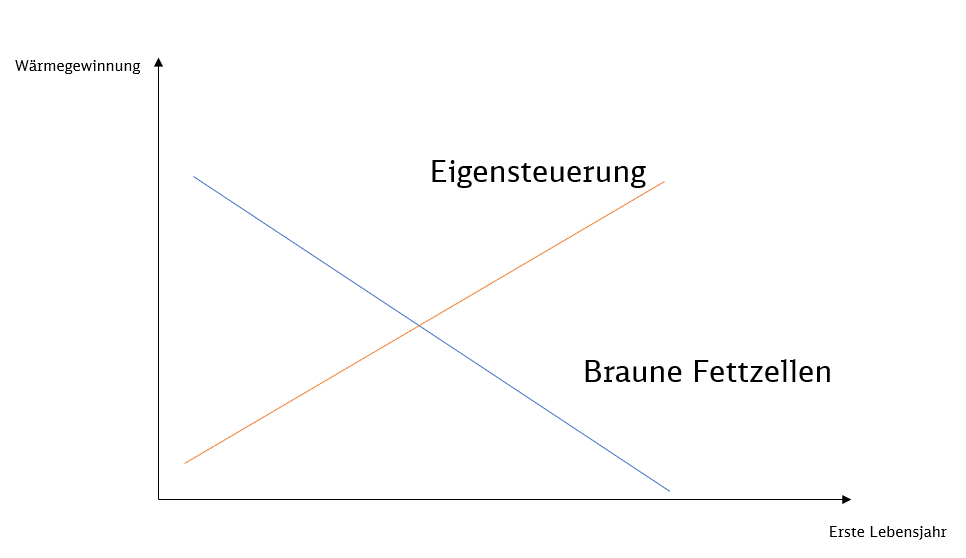
\includegraphics[scale = 0.3]{attachment/chapter_9/Scc001}
			\end{figure} 
		\end{itemize} \footnote{Empfehlung: Generell fühlen sich Säuglinge gut angezogen bei einer Raumtemperatur von etwa 24 bis 25 Grad Celsius am wohlsten. Herrschen aber in den Räumen der Wohnung „normale“ Temperaturen, das heißt zwischen 20 und 23 Grad Celsius im Wohnzimmer und 17 bis 20 Grad im Schlafzimmer, sind ein Body oder ein Shirt aus Baumwolle genau das Richtige zum Unterziehen für das Baby. Darüber eignet sich dann ein recht enganliegender leichter Pullover, beziehungsweise ein nicht allzu dickes Sweatshirt optimal.}
		\item Immunsystem
		\begin{itemize}
			\item Das Immunsystem wird bis das Stillen abgeschlossen ist, von der Muttermilch unterstützt. Antikörper werden über die Milch übertragen.
			\item Gleichzeitig trägt der enge Bund dazu bei, dass die Mutter den gleichen Erregern ausgesetzt ist.
		\end{itemize}
		\item Plötzlicher Kindstod
		\begin{itemize}
			\item Genaue physische Ursachen sind für dieses Phanomän sind nicht ableitbar.
			\item Empfehlungen wie: \textit{Säuglinge} im ersten Lebensjahr sollen immer auf dem Rücken einschlafen, und es soll kontrolliert werden, dass dies auch durch die Nacht hin passiert. Es ist dabei möglich, dass auf dem Bauch zuerst eingeschlafen wird und später der Säugling umgedreht wird. 
			\item Tagsüber ist für die Ausbildung der Rückenmuskulatur entscheidend, dass der Säugling auf dem Bauch liegt. 
		\end{itemize}
	\end{itemize}
	\item[0 Jahre - 6 Wochen]
	\begin{itemize}
		\item Iterationen mit unvertrauten Umgebungen sind eine hohe Lernherausforderung. Beispiel: Ein Besuch im Supermarkt zählt zu solchen Lerneindrücken.
		\item Die Hörqualität wird mit weiterem Alter nur noch abnehmen, und ist somit nie wieder so gut, wie als Neugeborenes.
		\item Retina und die Muskulatur zum Einstellen der Linse ist noch nicht entwickelt und trainiert. Diese führt dazu, dass schwarz-weiß und unscharf gesehen wird.
		\item Nach ca. 2 Monaten können Farben auseinander gehalten werden.
		\item Nach ca. 4 Monaten können Gesichter auseinander gehalten werden.
		\item In den ersten drei Monaten herrscht eine Wachstumsrate von 25 $\%$ je Monat.item Ab 6 Monaten kann sich ein Säugling meist drehen.
		\item Ab 6 Monaten kann sich ein Säugling meist drehen. Dies erhöht das Risiko für einen plötzlichen Kindstod.
	\end{itemize}
	\item[0 Jahre - 8 Monate]
	\begin{itemize}
		\item Alle Sinne sind vollständig ausgebildet.
		\item Mit dem Tastsinn werden weitere Lernprozesse angestoßen.
		\item Weil die Dichte im Mund an Sinneszellen sehr hoch ist, wird dieser genutzt, um eine höhere Lernqualität zu erhalten. Der Mund besitzt spezielle Enzyme, welche Bakterien angreifen.
		\item Mit dem 9 Lebensmonat startet die Aushärtung der Kopfform und Knochenbildung. Dies führt dazu, dass Asymetrien sich ab diesen Zeitpunkt verfestigen. Bis zum Ende des ersten Jahres ist dieser Prozess abgeschlossen.
	\end{itemize}
	\item[1 Jahr]
	\begin{itemize}
		\item Durch die Möglichkeit des Krabbels startet die Entwicklung von einem Baby zu einem Kleinkind.
		\item Fähigkeit des Sprechens wird entwickelt
	\end{itemize}
	\item[11 Jahren]
	\begin{itemize}
		\item Hormonbildung startet.
		\item Die sexuelle Entwicklung startet.
	\end{itemize}
\end{enumerate}
\footnote{
	Quelle 1: \href{https://www.ipzf.de/gehirnentwicklung.html}{Link},
	Quelle 2: \href{https://www.youtube.com/watch?v=ZNYv_ory8rc}{Living Body Documentation},
	Quelle 3: %\href{https://kinderzeit-bremen.de/familienzeit/schwanger-und-baby/waermehaushalt-bei-neugeborenen-tipps-risiken/#:~:text=Gerade\%20in\%20den\%20ersten\%20neun,kommt\%20es\%20rasch\%20zu\%20Temperaturverlust.}{Wärmehaushalt bei Neugeborenen}
	%Quelle 4: \href{https://www.varilag.de/ratgeber/baby-kopfform/#:~:text=Die\%20Sch\%C3\%A4delbasis\%20entwickelt\%20sich\%20aus,die\%20den\%20Sch\%C3\%A4del\%20flexibel\%20halten.}{Die Kopfform von Babys}
}



\subsubsection{Zeitlose Komponenten}
% was soll übermittelt werden: Selbst erlernte Strategien, welche von neuen 
% Thema: Eigenes Geld verdienen
% Wie wird umgegangen, bei Themen, welche noch nicht durchdacht sind: Dies werden angesprochen, dass über diese Entscheidugen oder Anreizstruktur noch keine eigenständige vollständige, gedankliche Endstruktur aufgebaut wurde.

\begin{itemize}
	\item $"$Mit den Geschenken der \gls{p_FM} schafft \gls{p_NFM} seinen eigenen Weg. Diese Geschenken können auch negativer Natur sein, da der gewünschte Effekt nicht eintritt. \textit{With all that is given to you, you make it your own (Marvel, Shing Chan)}
	\item Umgang mit Geld: Unklar, wie dies genau passen soll.
	\item Ein Ziel ist: Die Strategien, die von \gls{p_FM} selber erlernt wurden, dem \gls{p_NFM} zu vermitteln. Diese können vom \gls{p_NFM} angenommen, modifiziert oder auch abgeleht zu werden. 
	\item Ausbildung: Verweis: Conan $\&$ Harvard. Zwecke der Ausbildung. Es gibt Phasen der Ausbildung, in welcher das \gls{p_NFM} experimentieren soll, um zu lernen, worin es nicht gut ist und was ein wirklich reizt.
\end{itemize}

\end{comment}

% Referenz, wenn möglich
%%----- Maßnahme
%% - Unerreichbare Situation akzeptieren
%% - Fokus auf den eigenen Zustand, wenn extern nichts zu ändern ist.


% Von Zweier zu Dreier Dynamik zu Zweier Dynamik
Die Dynamik mit meiner Frau unterlag jetzt schon seit einigen Jahren einem Test zur Kalibrierung. Eingehen auf die Bedürfnisse des anderen, hat sich bis jetzt kein Ressentiment %französisch ausgesprochen
zueinander aufgebaut oder anderen negativen Effekten sich kumuliert. Mit dem Zuwachs von \gls{p_NFM} wird unsere zweier Dynamik sich zu einer dreier Dynamik ändern und ändern muss. Und mit dem Auszug von \gls{p_NFM} sich eine neue Form der zweier Dynamik bilden müssen.



\section{Die Aufteilung ist wie folgt:}
\begin{itemize}

	\item Gemeinsame Aufbau einer Familie. Transformation der Eltern und Kind Rolle 
	%%% Alle diese Kapitel werden aus NFM und unsere Ansicht betrachtet; Hier ist wichtig, dass NFM im weiteren Verlauf sich einbringt, und seinen Einschätzung mit einbringt.
	%%% 
	% Dynamik Eltern-NFM Beziehung (Analyse, Einwirkung); Verantwortungen und der Transfer von Verantwortung: Unser Ziel ist, dass NFM am Ende bis auf eine Ausnahmen (Absolute gefühlt Sicherheit in der Liebe) mit uns auf gleich auf ist in der Verwantung und ausprägung des eigenen Lebens.
	%% Hier spielt die Integration der Familie und Feunde in der Erziehung eine Rolle.
	% Erhaltung der Paar-Beziehung und Freundschaftbeziehungen
	%% Für uns als Paar ist es wichtiger, als für NFM, weil NFM diese noch im weiteren Verlauf wächsen lassen kann.
	%% Risiko-Umfeld
	% Einbettung von uns als Familie und uns selbst in das angrenzende Soziale Geflecht
	% Erhaltung der Paar-Beziehung
	% Energie-Haushalt
\end{itemize}

\section{Gemeinsame Familie}
Unser Ziel ist, dass jeder an dem Unterfangen Familie teilnimmt.\footnote{Dies axiomatisch. Es kann aber auch rationalisiert werdne.} 
% Reference zu Objectiv 






\section{Aufteilung}

\section{Objective} \label{part:NFM_sec:Objective}

Unser Ziel ist, dass wir als Familie gemeinsam und jeder von uns kontinuierlich daran arbeitet, dass wir eine eine \textit{tolle} Familie für einander sind.\\ 










welcher seinen eigenen Werte und Ziele verfolgen kann.

Mit allen was wir NFM geben, 


Soll es was eigenen daraus machen. 
Wir freuen uns zusehen, wenn wir es geschafft haben, einen selbstständigen Menschen zu erziehen, welcher eigene Wert und Ziele verfolgen kann (Unterschreiben)	


\begin{comment}
	Integrationsstrategie
	- Einleitung
	- NfM and I
	- Fundament Eltern schaffen
	- Stabiles Soziales Geflecht

Im zweiten Kapitel, kann Franziska ebenso eins hinzufügen.
, so I give it show and explain why Approach: Maybe a section, which explains
\end{comment}

Die Integration eines \gls{p_NFM} hat das Ziel, 
\begin{itemize}
	\item BSS bereichern $\&$ nicht gefährden
	\item Nach der vollständigen Deintegration ein größers soziales Familien/ Freunde Netzwerk bieten soll
\end{itemize}
%BSS - bestehende Soziale Strutkur (Freunde und Familie)

Die bestehende zwei-Familien-, die gesamthafte Familien- und Freundes Struktur  darunicht zu gefährden sondern zu bereichern sein.

% Die Hoffnung ist, dass NFM eine ganz eigenes Erlebnis im Leben für einen ist, weil diese Beziehung sonst nicht nachsimmuliert werden kann. BFM haben eine Verwantwortugn abnehmend gerichtete Beziehhungsstruktur. Dies soll umgedeht sein.

Unser Ziel ist, ein \gls{p_NFM} in unsere bestehende zwei-Familiestruktur zu integrieren. 
Am Ende sollen unser Zielsetzungen

\begin{comment}
	WDH und zum Warmwerden.
	Das Ziel ist, 
	eine tolle Familie
	- und super Freunde in eigenen Leben zu haben.

	Der Schritt mit der Erweiterung unsere eigenen Familien durch ein \gls{NFM} bringt Chance und Risiken mit sich. 
	
	Die Annahme besteht, dass dieser Schritt besonders große und langfristige Auswirken direkt so wie indirekt auf die genannten Zielsetzungen haben wird.
	
	
	Risiken, welche mit einer hohen Wahrscheinlichkeit antizipierbar sind, 
	
	
	Was benötigt es dafür: Das unterfangen eines NFM erfordert, dass wir lange durchhalten.
	
	
	Mit dem Zuwachs eder eigenen Familie, 
	entstehen Risiken, die durch dieses Unterfangen hervorgehen. Um diese abzufär
\end{comment}
\section{Stabiles Soziales Geflecht}
\section{Fundament Eltern und Paar}




% Offen
%Für wen: Uns drei und mögliche Freunde oder Familienangehörige.

\section{Lose}
% Zu löschen %%
Der Erfolg unser Familie soll daran bestehen, dass jeder von uns eine \textit{kontinuierliche} und \textit{liebende} Beziehung zu einandern führt, sodass wir über die individuellen Beziehungen hinaus eine Familie erschaffen: Mit Franziska und \gls{p_NFM} glücklich bis ans Ende meines Lebens zu sein, ist mein höchstes Priorität.\\

Der Strategie Name, \gls{p_NFM}, wurde aus zwei Gründen ausgewählt. Zum einen sollte eine so neutrale Ansicht wie möglich gewährleistet werden, zum anderen ist im ersten Draft Ansatz Kategorie wie \textit{Kind} und Jungentlicher zu kurzgekommen, bei der längeren Betrachtung. Die Neutralität rührte daher, dass im Vorfeld kein Attribute von \gls{p_NFM} im Vorfeld Einfluss auf uns nehmen soll, um die größte Entfaltungsmöglichkeit für \gls{p_NFM} gewährleisten zu können.\\


Unser Ziel ist es,
\begin{center}
dass wir mit \gls{p_NFM} die bestehende Familie erweitern und eine \textbf{tolle Familie} \underline{gemeinsam} aufbauen.	
\end{center}


\begin{itemize}
	\item ein integrierte Mitglied im bestehenden  erweiterten Familien- und teilweise in unserem Freundeskreis ist.
	\item Ebenso ist unser Ziel, dass wir selbständige Mitglieder  
	
	zu integrieren, sodass dieses Kreise auch Ihre Kreise sind.
\end{itemize}

Die folgenden Ausführen ist ein erster Versuch, bekannte Risiken zu adressieren und  Konsistenz in dem Maßnahmen bei der Zielerreichung auf dem Weg dahin zu geben.


\section{NFM and I}

\subsubsection{Dynamische Beziehung}
Die Annahme besteht, die Beziehungsdynamik zwischen \gls{p_NFM} und einem oder beiden Elternteilen durchläuft altersbezogene Phasen, welche durch die dominante Entwicklungsschritte im sozialen und physischen Bereich von \gls{p_NFM} angestoßen werden.

%TODO: Zielsetzung einfügen.
Um die 
Unter der Zielsetzung der Familie, ..., wird 

Der Umgang und die 

 in der Beziehungsdynamik bei einem Paar, das 

in einer Paar-Beziehung, in der Beziehung zu \gls{p_NFM} die soziale und physische Veränderung  der Änderung von \gls{p_NFM} 


Im Gegensatz zu der initalen Paar-Beziehung, sind die Entwicklungsschritte zum einen physisch und sozial in einer schnelleren Rate, als

Die Herausforderung wird sein, 

%0-3 Präsent
%3-8 Struktur Präsent, Elternrolle
%8-12 Eigene Intressen + Verantwortung
%12 - 18 Vollständiges Mitglied der Famiele, maximale Sicherheit, Gemeinsame Erlebnisse
% Referenzwert von Lotte-Entwicklung für die einzelnen Ebenen, um eine visuelle Hilfe zu geben.

\paragraph{Ab 0 Jahre}
\paragraph{Ab 1/2 Jahr}
\paragraph{Ab 1 Jahr}
- Elternrolle; Integration in den Familienablauf; 
\paragraph{Ab 6 Jahre}
- Ausbau eigener Interesse + Verantwortung für sich selbst
- Achten: Selbstbild
\paragraph{ab 10 Jahr}
\paragraph{ab 14 Jahre}
\paragraph{ab 18 Jahre}






Hier geht es darum, Eckpfeiler zu haben, welche wichtig sind, ,wann die Beziehung zu einander sich ändert.

\section{Kontinuierlich und liebende}
Die Erweiterung zu einer Familie bringt für uns als Paar nicht nur Chancen und Vorteile, sondern auch Risiken mit sich.\\


Damit dies gelingt, sehen setzen wir die folgenden Schwerpunkte:

\paragraph{Fundament Eltern / Paar-Beziehung}

Für uns als Paar, als Teil der Familie, ist uns wichtig, dass in der Einbettung zur Familie wir die Paar-Beziehung nicht verloren geht und wir weiterhin eine \textit{kontinuierliche} und \textit{liebende} Paarbeziehung führen können.\\

Themen welche jetzt schon erkannt werden, dem im Wege zu stehen, werden in diesem Abschnitt adressiert.


\paragraph{Stabiles Soziales Geflecht} Wir als Paar haben bisher einen Schwerpunkt auf tolle Freunde und eine super Familie gelegt. Dies bedeutet, dass wir Zeit investiert haben, uns mit Freunden und Familie\footnote{In dem Kontext ist die erweiterte Familie gemeint, in derm man selbst ein \gls{p_NFM} war oder in einer andere indirekten Beziehung steht.} zu treffen, um gemeinsame Erlebnisse zu schaffen.\\

In diesem Abschnitt wird ausgeführt, wir dies als Familie ermöglicht werden kann.

\paragraph{NFM and I}
Die Beziehung zu \gls{p_NFM} wird anderen Schwerpunkt beinhalten müssen, als bisherige andren soziale Beziehungen.\\

Alle Themen, welche die Beziehung eines selbst als Elternteil zu \gls{p_NFM} versuchen zu adressieren, werden hier ausgeführt.



